\chapter{Appendix B: Examples of Assessment Items}
\vspace{-.53in}
   \noindent\color{graylight}\rule[0cm]{3.25in}{0.03cm} \\
    \noindent\color{graylight}\rule[0.4cm]{3.25in}{0.03cm} \\
\color{black}






\added{\newthought{Well-designed assessment items} help to determine whether students understand key statistical concepts.  Since the original GAISE report was written in 2005, there have been many improvements in the ways that instructors and institutions determine whether students have met the learning outcomes for introductory statistics courses.  

Students value that which is assessed, 
\marginnote{\textit{In general, we want students to interpret results more than we want them to produce results. If we ask a True/False question, we want the student to explain \emph{why} a statement is true or is false, so that we can assess the thinking that lead to the answer chosen. However, sometimes the practicalities of teaching a large class mean that an appropriate exam question might be a multiple choice item that does not ask for explanation.}}
so it is important that we assess student learning in a manner consistent with our stated goals. Good items assess the development of statistical thinking and conceptual understanding, preferably using technology and real data.

Below we present exemplary assessment items, some of which include commentary. We also present a few items that are not strong, with suggestions on how they can be improved. Finally, we present advice on constructing a rubric when assessing a project report or presentation.

}

\section{\textbf{\added{Examples of Exemplary Assessment Items}}}
\added{We begin by providing examples of exemplary assessment items with commentary about the items.}

\subsection{\textbf{\textit{\added{Item -6}}}}
\added{Are metal bands used for tagging harmful to penguins?}
\marginnote{\added{\textit{XX add commentary here...}}}
\added{Researchers investigated this question with a sample of 100 penguins near Antarctica.  All of these penguins had already been tagged with RFID chips, and the researchers randomly assigned 50 of them to receive a metal band on their flippers in addition to the RFID chip. The other 50 penguins did not receive a metal band. Researchers then kept track of which penguins survived for the 4.5-year study and which did not.  They found that 16 of the 50 penguins with a metal band survived, compared to 31 of the 50 penguins without a metal band.  
\begin{enumerate} [leftmargin=1cm, itemsep=.2em]
\item Calculate the difference in the proportions who survived between the two groups.

\item The p-value for comparing the two group's survival proportions turns out to be .002.
Explain (as if to someone who has not studied statistics) what this p-value means: This is the probability of $\ldots$

\item Summarize your conclusion from this p-value.  Be sure to address the issue of causation as well as the issue of significance.  Also justify your conclusion.
\end{enumerate}
}


\subsection{\textbf{\textit{\added{Item -5}}}}
\added{Suppose that 20\% of undergraduate students at a university own an iPad and 60\% of graduate students at the university own an iPad.  Is it reasonable to conclude that 40\% (the average of 20\% and 60\%) of all students at the university (undergraduate and graduate students combined) own an iPad?  Explain why or why not, as if to a college student who has not taken a statistics class.}


\subsection{\textbf{\textit{\added{Item -4}}}}
\added{Suppose that you take a random sample of 100 houses currently for sale in California.  Does the Central Limit Theorem suggest that a histogram of the house prices in the sample will display an approximately normal distribution?  Explain briefly.}

\subsection{\textbf{\textit{\added{Item -3}}}}
\added{Does everyone who scores below the median on this exam necessarily have a negative z-score for this exam?  Explain.}

\subsection{\textbf{\textit{\added{Item -2}}}}
\added{Describe a situation}
\marginnote{\added{\textit{Sample solution: For an observational study which assessed the association between coffee drinking and cancer, smoking status could mask (or ``confound") the relationship, since smoking could be associated with both coffee drinking and cancer.}}}%
\added{where a third variable could be masking the relationship between two variables.  }

\subsection{\textbf{\textit{Was Old Item 8}}}
Let Y denote the amount a student spends on textbooks for one semester. Suppose Nancy, who is statistically savvy, wants to know how fall, semester 1, and spring, semester 2, compare.  In particular, suppose she is interested in the averages ?1 and ?2.  You may assume that Nancy has taken several statistics courses and knows a lot about statistics, including how to interpret confidence intervals and hypothesis tests.  You have random samples from each semester and are to analyze the data and write a report.  You seek advice from four persons:

\begin{enumerate}[leftmargin=1cm, itemsep=.2em]
\item \textbf{Rudd says,} ``Conduct an $\alpha=.05$ test of $H_0: \mu_1=\mu_2$ vs. $H_A: \mu_1 \neq \mu_2$ and tell Nancy whether you reject $H_0$.''

\item \textbf{Linda says,} ``Report a 95\% confidence interval for $?_1 - ?_2$ .''


\item \textbf{Steve says,} ``Conduct a test of $H_0: \mu_1=\mu_2$ vs. $H_A: \mu_1 \neq \mu_2$ and report to Nancy the \textit{p}-value from the test.''

\item \textbf{Gloria says,} ``Compare $\bar{y}_1$  to $\bar{y}_2$.  If $\bar{y}_1 > \bar{y}_2$,  then test $H_0: \mu_1=\mu_2$ vs. $H_A: \mu_1 > \mu_2$ using $\alpha =.05$ and tell Nancy whether you reject $H_0$.  If $\bar{y}_1 < \bar{y}_2$,  then test $H_0: \mu_1=\mu_2$ vs. $H_A: \mu_1 < \mu_2$ using $\alpha = .05$ and tell Nancy whether you reject $H_0$.''
\end{enumerate}

Rank the four pieces of advice from worst to best and explain why you rank them as you do. That is, explain what makes one better than another.


\section{\textbf{Examples of Assessment Items with Problems and Commentary \deleted{About the Nature of the Difficulty}}}
We \replaced{next}{first} give some examples of assessment items with problems and commentary about the nature of the difficulty.

\vspace{8pt}

\textbf{\textit{Assessment items to avoid using on tests: \added{traditional} True/False, pure computation without a context or interpretation, items with too much data to enter and compute or analyze, \added{or} items that only test memorization of definitions or formulas.}}

\subsection{\textbf{\textit{Item 1}}}
A teacher taught two sections \marginnote{\textit{Critique: The teacher has all the population data so there is no need to do statistical inference. \added{In addition, the proposed design has serious flaws in terms of statistical practice.}}}of elementary statistics last semester, each with 25 students, one at 8:00 a.m. and one at 4:00 p.m. The means and standard deviations for the final exams were 78 and 8 for the 8:00 a.m. class and 75 and 10 for the 4:00 p.m. class. In examining these numbers, it occurred to the teacher that the better students probably sign up for 8:00 a.m. class. So she decided to test whether the mean final exam scores were equal for her two groups of students. State the hypotheses and carry out the test.

 

\subsection{\textbf{\textit{Item 2}}}
An economist wants to compare \marginnote{\textit{Critique: The question doesn't address the conditions necessary for a \textit{t}-test, and with the small sample sizes, they are almost surely violated here. Salaries are almost surely skewed.}} the mean salaries for male and female CEOs. He gets a random sample of 10 of each and does a \textit{t}-test. The resulting \textit{p}-value is .045.
\begin{enumerate} [leftmargin=1cm, itemsep=.2em]

\item State the null and alternative hypotheses.
\item Make a statistical conclusion.
\item State your conclusion in words that would be understood by someone with no training in statistics.
\end{enumerate}



\subsection{\textbf{\textit{Item 3}}}
Which of the following gives the definition of a \textit{p}-value?
\renewcommand{\labelenumi}{\Alph{enumi}.}
\begin{enumerate} [leftmargin=1cm, itemsep=.2em]
\marginnote{\textit{Critique: None of these answers is quite correct. Answers B and D are clearly wrong; answer A is the level of significance; and answer C would be correct if it continued ``\ldots  or more extreme, given that the null hypothesis is true.''}}
\item It's the probability of rejecting the null hypothesis when the null hypothesis is true.
\item It's the probability of not rejecting the null hypothesis when the null hypothesis is true.
\item It's the probability of observing data as extreme as that observed.
\item It's the probability that the null hypothesis is true.
\end{enumerate}



\section{\textbf{Examples Showing Ways to Improve Assessment Items}}
\added{\subsection{\textbf{\textit{Item 3 (revisited)}}}
Which of the following gives the definition of a \textit{p}-value?
\vspace{8pt}

\noindent\smallcaps{Changed to:} \\
 A randomized trial of the}
\marginnote{\added{\textit{Sample solution: If bednets were not associated with malaria prevalence then we'd only be likely to see a result this extreme or more extreme one time out of a thousand.  Therefore we conclude that bednets must be effective in preventing malaria.}}}
\added{use of bednets to prevent malaria in sub-Saharan Africa yielded a p-value of 0.001.  Without resorting to jargon, interpret this result in the context of the problem to someone without background knowledge of statistics.}

\vspace{8pt}
\textbf{\textit{True/False items, even when well-written, do not provide much information about student knowledge because there is always a 50\% chance of getting the item right without any knowledge of the topic. One \deleted{current} approach is to change the items into forced-choice questions with three or more options.}}

\subsection{\textbf{\textit{Item 4}}}
The size of the standard deviation of a data set depends on where the center is. True or False\\
\vspace{8pt}

\noindent\smallcaps{Changed to:} \\
 Does the size of the standard deviation of a data set depend on \\ \indent where the center is located?
\begin{enumerate} [leftmargin=1.5cm, itemsep=.2em]
\item Yes, the higher the mean, the higher the standard deviation.
\item Yes, because you have to know the mean to calculate the standard deviation.
\item No, the size of the standard deviation is not affected by the location of the distribution.
\item No, because the standard deviation only measures how the values differ from each other, not how they differ from the mean.
 \end{enumerate}


\subsection{\textbf{\textit{Item 5}}}
A correlation of $+1$ is stronger than a correlation of $-1$. True or False\\
\vspace{8pt}

\noindent\smallcaps{Rewritten as:}

A recent article in an educational research journal reports a \\ correlation of  $+0.8$ between math achievement and overall math \\ aptitude. It also reports a correlation of  $-0.8$ between math\\ achievement and a math anxiety test. Which of the following\\ interpretations is the most correct?
\begin{enumerate} [leftmargin=2cm, itemsep=.2em]
\item The correlation of $+0.8$ indicates a stronger relationship than the correlation of $-0.8$.
\item The correlation of $+0.8$ is just as strong as the correlation of $-0.8$.
\item It is impossible to tell which correlation is stronger.
\end{enumerate}

\noindent \textbf{\textit{Context is important for helping students see and deal with statistical ideas in real-world situations.}}

\subsection{\textbf{\textit{Item 6}}}
Once it is established that X and Y are highly correlated, what type of study needs to be done to establish that a change in X causes a change in Y?\\

\vspace{8pt}
\noindent\smallcaps{A context is added:}

A researcher is studying the relationship between an experimental \\ medicine and T4 lymphocyte cell levels in HIV/AIDS patients. \\ The T4 lymphocytes, a part of the immune system, are found at \\ reduced levels in patients with the HIV infection. Once it is \\ established that the two variables, dosage of medicine, and T4 cell \\ levels are highly correlated, what type of study needs to be done \\ to establish that a change in dosage causes a change in T4 cell \\levels? 
\begin{enumerate} [leftmargin=2cm, itemsep=.2em]
\item correlational study
\item controlled experiment
\item prediction study
\item survey
\end{enumerate}

\noindent\textbf{\textit{Try to avoid repetitious/tedious calculations on exams that may become the focus of the problem for the students at the expense of concepts and interpretations.}}

\subsection{\textbf{\textit{Old Item 21}}}
It was claimed 
\marginnote{\added{\textit{Critique: This problem requires use of software to calculate the exact binomial or use of the binomial approximation to the normal.  Computer output might be provided to augment this question and facilitate solution.}}}
that 1 out of 5 cardiologists takes an aspirin a day to prevent hardening of the arteries.  Suppose the claim is true.  If 1,500 cardiologists are selected at random, what is the probability that at least 275 of the 1,500 take an aspirin a day? 

\subsection{\textbf{\textit{Item 7}}}

A first-year program course \marginnote{\textit{Critique: The version of the question above requires a fair amount of pounding on the calculator to get the results and never even asks for an interpretation.  The revision below still requires some calculation (which can be adjusted depending on the amount of computer output provided) but the calculations can be done relatively efficiently---especially by students who have a good sense of what the computer output is providing.}} used a final exam that contained a 20-point essay question asking students to apply Darwinian principles to analyze the process of expansion in major league sports franchises.  To check for consistency in grading among the four professors in the course, a random sample of six graded essays were selected from each instructor.  The scores are summarized in the table below.  Construct an ANOVA table to test for a difference in means among the four instructors. 


\begin{table}[!ht]
\begin{center}
\begin{tabular}{lllllll}
\textbf{Instructor} & \multicolumn{6}{c}{\textbf{Scores}}\\
  \hline
Affinger & 18 & 11 & 10 & 12 & 15 & 12\\
Beaulieu & 14 & 14 & 11 & 14 & 11 & 14\\
Cleary & 19 & 20 & 15 & 19 & 19 & 16\\
Dean & 17 & 14 & 17 & 15 & 18 & 15\\
\hline
\end{tabular}
\end{center}
\end{table}



A first-year program course \ldots  (same intro as above) \ldots   The scores are summarized in the table below, along with some descriptive statistics for the entire sample and a portion of the one-way ANOVA output.




\begin{table}[ht]
\begin{center}
\begin{tabular}{lrrrrrr}

\multicolumn{7}{l}{\texttt{Descriptive Statistics}}\\
\texttt{Variable} & \texttt{N} & \texttt{Mean} & \texttt{Median} & \texttt{TrMean} & \texttt{StDev}  & \texttt{SEMean}\ \\ 

\texttt{Score} & \texttt{24.00} & \texttt{15.00} & \texttt{15.00} & \texttt{15.00} & \texttt{2.92}  & \texttt{0.60} \\ 
\\
\multicolumn{7}{l}{\texttt{One-way Analysis of Variance}}\\
& \multicolumn{6}{l}{\textit{***ANOVA TABLE OMITTED ***}}
\\
\\

\texttt{Level} & \texttt{N} & \texttt{Mean} & \texttt{StDev} & & &\\ 

\texttt{Affinger} & \texttt{6} & \texttt{13.00} & \texttt{2.97} & & & \\ 
\texttt{Beaulieu} & \texttt{6} & \texttt{13.00} & \texttt{1.55} & & & \\ 
 \texttt{Cleary} & \texttt{6} & \texttt{18.00} & \texttt{2.00} & & & \\ 
\texttt{Dean} & \texttt{6} & \texttt{16.00} & \texttt{1.55} & & & \\ 
  \\
\multicolumn{7}{l}{\texttt{Pooled StDev = 2.098}}\\


\end{tabular}
\end{center}
\end{table}


\begin{figure}
%\centering
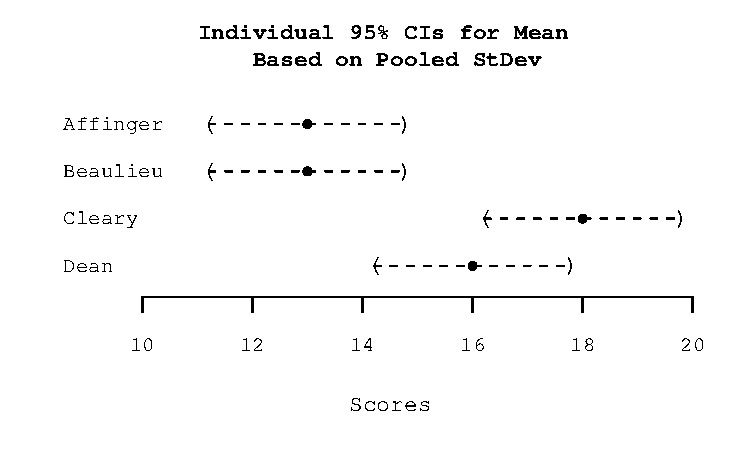
\includegraphics[width=3.5in]{includes/Item7_R.pdf}
\end{figure}

\renewcommand{\labelenumi}{\arabic{enumi}.}
\begin{enumerate}[leftmargin=1cm, itemsep=.2em]
\item Unfortunately, we are missing the ANOVA table from the output. Use the information given above to construct the ANOVA table and conduct a test (5\% level) for any significant differences among the average scores assigned by the four instructors.  Be sure to include hypotheses and a conclusion.   If you have trouble getting one part of the table that you need to complete the rest (or the next question), make a reasonable guess or ask for assistance (for a small point fee). 
\item After completing the ANOVA table, construct a 95\% confidence interval for the average score given by Dr. Affinger. \textit{Note: Your answer should be consistent with the graphical display.}
\end{enumerate}


\section{\textbf{Additional Examples of Good Assessment Items}}

\subsection{\textbf{\textit{\added{New Item 8}}}}
\added{A study found that individuals who lived in houses with more than two bathrooms tended to have higher blood pressure than individuals who lived in houses with two or fewer bathrooms.  Can cause-and-effect be determined from this?}

\subsection{\textbf{\textit{Item 9}}}
Researchers took random samples of subjects from two populations and applied a \deleted{Wilcoxon-Mann-Whitney} test to the data; the \textit{P}-value for the test, using a nondirectional alternative, was .06.  For each of the following, say whether the statement is true or false and why.
\begin{enumerate}[leftmargin=1cm, itemsep=.2em]
\item There is a 6\% chance that the two population distributions really are the same.
\item If the two population distributions really are the same, then a difference between the two samples as extreme as the difference that these researchers observed would only happen 6\% of the time.
\item If a new study were done that compared the two populations, there is a 6\% probability that $H_0$ would be rejected again.
\item If $\alpha = .05$ and a directional alternative were used, and the data departed from $H_0$ in the direction specified by the alternative hypothesis, then $H_0$ would be rejected.
\end{enumerate}

\subsection{\textbf{\textit{Item 10}}}
An article on the CNN web page \deleted{(\url{www.cnn.com/HEALTH/9612/16/faith.healing/index.html})} \deleted{on Monday} begins with the sentence, ``Family doctors overwhelmingly believe that religious faith can help patients heal, according to a survey released Monday.''  Later, the article states, ``Medical researchers say the benefits of religion may be as simple as helping the immune system by reducing stress,'' and Dr. Harold Koenig is reported to say that ``people who regularly attend church have half the rate of depression of infrequent churchgoers.''
  
Use the language of statistics to critique the statement by Dr.\ Koenig and the claim, suggested by the article, that religious faith and practice help people fight depression. You will want to select some of the following words in your critique: observational study, experiment, blind, double-blind, precision, bias, sample, spurious, confounding, causation, association, random, valid, reliable.

\subsection{\textbf{\textit{Item 11}}}
\replaced{A student}{Francis (Class of '18)} weighed 100 Hershey's Kisses (with almonds).  She found that the sample average was 4.80 grams and the SD was .28 grams. \textit{In the context of this setting,} explain what is meant by the sampling distribution of an average.

\subsection{\textbf{\textit{Item 12}}}
A gardener wishes to compare the yields of three types of pea seeds---type A, type B, and type C.  She randomly divides the type A seeds into three groups and plants some in the east part of her garden, some in the central part of the garden, and some in the west part of the garden.  Then, she does the same with the type B seeds and type C seeds.
\begin{enumerate}[leftmargin=1cm, itemsep=.2em]
\item \textit{What kind} of experimental design is the gardener using?
\item \textit{Why} is this kind of design used in this situation?  (Explain in the \textit{context of the situation.})
\end{enumerate}

\subsection{\textbf{\textit{Item 13}}}
The scatterplot shows how divorce rate, y, and marriage rate, x, are related for a collection of 10 countries.  The regression line has been added to the plot.

\begin{marginfigure}
\centering
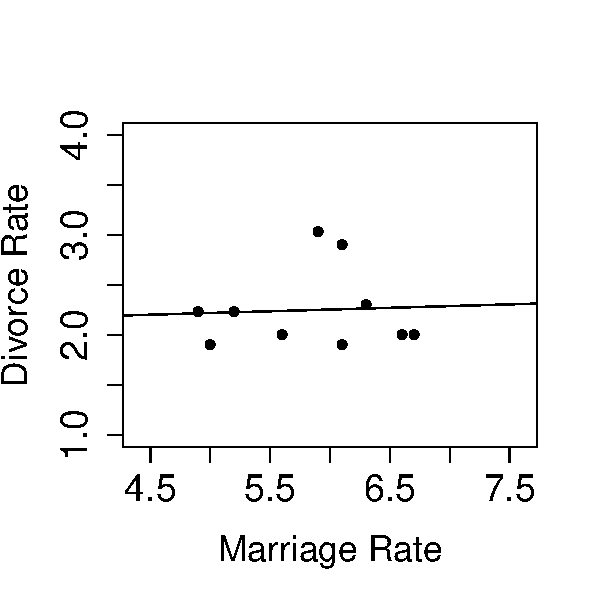
\includegraphics{includes/Item13_R.pdf}
\end{marginfigure}

\begin{enumerate}[leftmargin=1cm, itemsep=.2em]
\item The U.S. is not one of the 10 points in the original collection of countries.  It happens that the U.S. has a higher marriage rate than any of the 10 countries.  Moreover, the divorce rate for the U.S. is higher than one would expect, given the pattern of the other countries.  How would adding the U.S. to the data set affect the regression line?  Why?
\item Think about the scatterplot and regression line after the U.S. has been added to the data set.  Provide a sketch of the residual plot.  Label the axes and identify the U.S. on your plot with a triangle.
\end{enumerate}


\subsection{\textbf{\textit{Item 14}}}
Researchers wanted to compare two drugs, formoterol and salbutamol, in aerosol solution to a placebo for the treatment of patients who suffer from exercise-induced asthma.  Patients were to take a drug or the placebo, do some exercise, and then have their ``forced expiratory volume'' measured.  There were 30 subjects available. (Based on A.N. Tsoy, et al., \textit{European Respiratory Journal 3} (1990): 235; via Berry, \textit{Statistics: A Bayesian Perspective}.)
\begin{enumerate}[leftmargin=1cm, itemsep=.2em]
\item Should this be an experiment or an observational study?  Why?
\item Within the context of this setting, what is the placebo effect?
\item Briefly explain how to set up a randomized blocks design (RBD) here.
\item How would an RBD be helpful?  That is, what is the main advantage of using an RBD in a setting like this?
\end{enumerate}

\subsection{\textbf{\textit{\deleted{Item 15}}}}
\deleted{I noticed that eight students from the 114 class attended the review session prior to the second exam (in April).  The average score among those eight students was lower than the average for the 21 students who did not attend the review session.  Suppose I want to use this information in a study of the effectiveness of review sessions.}
\begin{enumerate}[leftmargin=1cm, itemsep=.2em]
\item \deleted{What kind of study is this, observational or experimental?  Why?}
\item \deleted{What kind(s) of sampling error(s) or bias(es) might be of concern here?}
\item \deleted{(Hypothetical)  I gave the data for the eight who attended and for the 21 who did not attend to my friend George.  George used the data to conduct a hypothesis test.  Does a hypothesis test make sense?  If so, what is $H_0$?  If not, why not?}
\end{enumerate}



\subsection{\textbf{\textit{Item 16}}}
For each of the following three settings, state the type of analysis you would conduct (e.g., one-sample \textit{t}-test, regression, chi-square test of independence, chi-square goodness-of-fit test, etc.) if you had all the raw data and specify the roles of the variable(s) on which you would perform the analysis, but \textit{do not actually carry out the analysis}.
\begin{enumerate}[leftmargin=1cm, itemsep=.2em]
\item \replaced{A student}{Elizabeth Larntz (Class of '02)} measured the effect of exercise on pulse for each of 13 students.  She measured pulse before and after exercise (doing 30 jumping jacks) and found that the average change was 55.1 and the SD of the changes was 18.4.  How would you analyze the data?
\item Three HIV treatments were tested for their effectiveness in preventing progression of HIV in children.  Of 276 children given drug A, 259 lived and 17 died. Of 281 children given drug B, 274 lived and seven died.  Of 274 children given drug C, 264 lived and 10 died.  How would you analyze the data?
\item \replaced{A researcher was interested in the relationship between blood pressure and physical activity.}{A researcher was interested in the relationship between forearm length and height.}
\replaced
{He measured the blood pressure and weekly total number of steps from a Fitbit for 125 women.}  
{He measured the forearm lengths and heights of each of 16 women.}
How would you analyze these data?
\end{enumerate}

\subsection{\textbf{\textit{Item 17}}}
I \replaced{constructed}{had Data Desk construct}
parallel dotplots of the data from four samples.  I then conducted a test of $H_0: \mu_1=\mu_2=\mu_3=\mu_4$ and rejected $H_0$ at the $\alpha = .05$ level.  I also tested $H_0: \mu_1=\mu_2=\mu_3$ and rejected $H_0$ at the $\alpha = .05$ level.  However, when I tested $H_0: \mu_2=\mu_3$ using $\alpha = .05$, I did \textit{not} reject $H_0$.  Likewise, when I tested $H_0: \mu_1=\mu_4$ using $\alpha = .05$, I did \textit{not} reject $H_0$.
\begin{enumerate}[leftmargin=1cm, itemsep=.2em]
\item Your job is to sketch a graph of the parallel dotplots of the data. That is, based on what I told you about the tests, you should have an idea of how the data look. Use that idea to draw a graph.  Indicate the sample means with triangles that you add to the dotplots.
\item It is possible to get data with the same sample means that you graphed in part 1, but for which the hypothesis $H_0: \mu_1=\mu_2=\mu_3=\mu_4$ is not rejected at the $\alpha = .05$ level.  Provide a graph of this situation.  That is, keep the same sample means (triangles) you had from part 1, but show how the data would have been different if $H_0$ were not to be rejected.
\end{enumerate}

\subsection{\textbf{\textit{Item 18}}}
\replaced{A student}{Atley Chock (Class of `02)} collected data on a random sample of 12 breakfast cereals.  \replaced{They}{He} recorded x = fiber (in grams/ounce) and y = price (in cents/ounce).  A scatterplot of the data shows a linear relationship.  The fitted regression model is

\begin{equation*}
\hat{y} = 17.42 + 0.62x
\end{equation*}
  
The sample correlation coefficient, $r$, is 0.23.  The SE of $b_1$ is .81.   Also, $s_{y|x}$ = 3.1.
\begin{enumerate}[leftmargin=1cm, itemsep=.2em]
\item Find $r^2$ and interpret $r^2$ in the context of this problem.
\item Suppose a cereal has 2.63 grams of fiber/ounce and costs 17.3 cents/ounce.  What is the residual for this cereal?
\item Interpret the value of $s_{y|x}$ in the context of this problem.  That is, what does it mean to say that $s_{y|x}$ = 3.1?
\item In the context of this problem, explain what is meant by ``the regression effect.''
\end{enumerate}

\subsection{\textbf{\textit{Item 19}}}
Give a rough estimate of the sample correlation for the data in each of the scatterplots below.

\begin{figure}[ht]
\centering
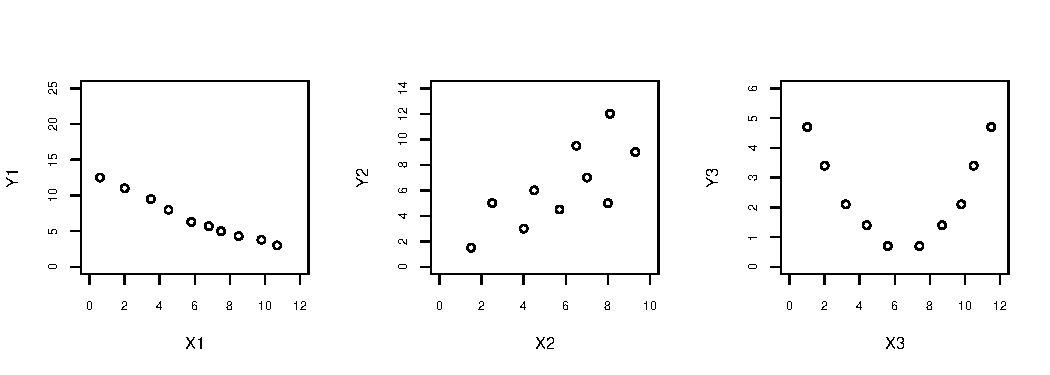
\includegraphics[width=6.5in]{includes/Item19_R.pdf}
\end{figure}


\subsection{\textbf{\textit{\deleted{Item 20}}}}
\deleted{A matched pairs experiment compares the taste a regular cheese pizza of Pizza Joe's to Domino's.  Each subject tastes two unmarked pieces of pizza, one of each type, in random order and states which he or she prefers.  Of the 50 subjects who participate in the study, 21 prefer Pizza Joe's.   }
\begin{enumerate}[leftmargin=1cm, itemsep=.2em]
\item \deleted{Find a 96\% confidence interval for the proportion of the population that prefers Pizza Joe's to Domino's.}
\item \deleted{How large a sample is required if the desired margin of error of the confidence interval is 4\%?}
\end{enumerate}

\subsection{\textbf{\textit{Item 22}}}
Identify whether a scatterplot would or would not be an appropriate visual summary of the relationship between the variables.  In each case, explain your reasoning.  
\begin{enumerate}[leftmargin=1cm, itemsep=.2em]
\item Blood pressure and age
\item Region of country and opinion about stronger gun control laws
\item Verbal SAT and math SAT score
\item Handspan and gender (male or female)
\end{enumerate}

\subsection{\textbf{\textit{Item 23}}}
The paragraphs that follow each describe a situation that calls for some type of statistical analysis.  For each, you should:
\renewcommand{\labelenumi}{\arabic{enumi}.}
\begin{enumerate}[leftmargin=1cm, itemsep=.2em]
\item Give the name of an appropriate statistical procedure to apply (from the list below). You may use the same procedure more than once, and some questions might have more than one correct answer.
\item In some problems, you will also be given a \textit{p}-value. Use it to reach a conclusion for that specific problem.  Be sure to say something more than just Reject $H_0$ or Fail to Reject $H_0$. (Assume a 5\% significance level.) 
\end{enumerate}

Some statistical procedures you might choose:
\begin{table}[!ht]
\begin{center}
\begin{tabular}{ll}
\hline
Confidence interval (for a mean, p, \ldots) & Normal distribution\\
Determining sample size	& Correlation\\
Test for a mean	 & Simple linear regression\\
Test for proportion & Multiple regression\\
Difference in means (paired data) & Two-way table (chi-square test)\\
Difference in means (two independent samples) & ANOVA for difference in means\\
Difference in proportions & Two-way ANOVA for means\\
\hline
\end{tabular}
\end{center}
\end{table}

\renewcommand{\labelenumi}{\Alph{enumi}.}

\begin{enumerate}[leftmargin=1cm, itemsep=.2em]
\item Anthropologists have found two burial mounds in the same region. They know several tribes lived in the region and that the tribes have been classified according to different lengths of skulls. They measure a random sample of skulls found in each burial mound and wish to determine if the two mounds were made by different tribes.  (\textit{p}-value = 0.0082) 

\bigskip
	
\item The Hawaiian Planters Association is developing three new strains of pineapple (call them A, B, and C) to yield pulp with higher sugar content. Twenty plants of each variety (60 plants in all) are randomly distributed into a two-acre field. After harvesting, the resulting pineapples are measured for sugar content and the yields are recorded for each strain.  Are there significant differences in average sugar content between the three strains? (\textit{p}-value = 0.987)
\bigskip	
\item Researchers were commissioned by the Violence In Children's Television Investigative Monitors (VICTIM) to study the frequency of depictions of violent acts in Saturday morning TV fare.  They selected a random sample of 40 shows that aired during this time period over a 12-week period.  Suppose 28 of the 40 shows in the sample were judged to contain scenes depicting overtly violent acts.  How should they use this information to make a statement about the population of all Saturday morning TV shows?
\bigskip	
\item The Career Planning Office is interested in seniors' plans and how they might relate to their majors.  A large number of students are surveyed and classified according to their MAJOR (Natural Science, Social Science, Humanities) and FUTURE plans (Graduate School, Job, Undecided).  Are the type of major and future plans related?  (\textit{p}-value = 0.047)
\bigskip
\item \textit{Sophomore Magazine} asked a random sample of 15 year olds if they were sexually active (yes or no).  They would like to see if there is a difference in the responses between boys and girls.     (\textit{p}-value = 0.029)
\bigskip	
\item Every week during the Vietnam War, a body count (number of enemy killed) was reported by each army unit. The last digits of these numbers should be fairly random.  However, suspicions arose that the counts might have been fabricated.  To test this, a large random sample of body count figures was examined and the frequency with which the last digit was a 0 or a 5 was recorded.  Psychologists have shown that people making up their own random numbers will use these digits less often than random chance would suggest (i.e., 103 sounds like a more ``real" count than 100).  If the data were authentic counts, the proportion of numbers ending in 0 or 5 should be about 0.20.  (\textit{p}-value=0.002)
\bigskip	
\item In one of his adventures, Sherlock Holmes found footprints made by the criminal at the scene of a crime and measured the distance between them. After sampling many people, measuring their height and length of stride, he confidently announced that he could predict the height of the suspect. How?
\end{enumerate}


\added{\subsection{\textbf{\textit{New Item 23B}}}}
\added{Some of the statistical inference techniques we have studied include:
\begin{description}
\item[A.]	One-sample z-procedures for a proportion
\item[B.]	Two-sample z-procedures for comparing proportions
\item[C.] 	One-sample t-procedures for a mean
\item[D.]	Two-sample t-procedures for comparing means
\item[E.]	Paired-sample t-procedures
\item[F.] 	Chi-square procedures for two-way tables
\item[G.]	ANOVA procedures
\item[H.]	Linear regression procedures
\end{description}

For each of the following research questions (on the next page), indicate (by letter) the appropriate statistical inference procedure for investigating the question.
\marginnote{\textit{The list of methods or examples can be shortened.}}
\begin{enumerate} [leftmargin=1cm, itemsep=.2em]
\item Economists compared starting salaries of new employees across three different groups: those with graduate degrees, those with only bachelor’s degrees, and those with no higher education degrees.

\item A researcher investigated whether laughter increases blood flow by having subjects watch a humorous movie and a stressful movie, randomly deciding which movie the subject would see first, measuring the blood flow through the person’s blood vessels while watching the movie.

\item Student researchers investigated whether balsa wood is less elastic after it has been immersed in water.  They took 44 pieces of balsa wood and randomly assigned half to be immersed in water and the other half not to be.  They measured the elasticity by seeing how far (in inches) the piece of wood would project a dime into the air.

\item Do more than two-thirds of students at a particular university have at least one class on Fridays during this term?

\item Are people more likely to fill in the missing letter in F A I \_ with an L if they are given a red pen rather than a blue pen?

\item Is there an association between a college student’s level of drinking alcohol (classified as none, some, or considerable) and her/his residence situation (classified as living on-campus, off-campus with parents, or off-campus but not with parents)?

\item A researcher used data from the American Time Use Survey (ATUS) to investigate whether high school math teachers tend to spend more time working per day than high school history teachers.

\item Biologists recorded the frequency of a cricket’s chirps (in chirps per minute) and also the temperature (in degrees Fahrenheit) when the cricket measurement was recorded.  They investigated whether chirp frequency is a significant predictor of temperature.
\end{enumerate}
}
 

\subsection{\textbf{\textit{Item 24}}}
How accurate are radon detectors of a type sold to homeowners?  To answer this question, university researchers placed 12 detectors in a chamber that exposed them to 105 picocuries per liter of radon.  The detector readings found are below.  A printout of the descriptive statistics from Minitab follows. 

\marginnote{\added{XX could we provide more output (e.g., 95\% confidence interval?) to allow testing without calculation or use of a table?}}

\begin{table}[!ht]
\begin{center}
\begin{tabular}{llllll}
91.9	& 97.8 & 111.4 & 122.3 & 105.4 & 95.0\\
103.8 & 99.6 & 96.6 & 119.3 & 104.8 & 101.7\\
\end{tabular}
\end{center}
\end{table}

\begin{table}[!ht]
\begin{center}
\begin{tabular}{lllllllllll}
\texttt{Variable} & \texttt{N} & \texttt{Mean} & \texttt{Median} &    \texttt{TrMean} & \texttt{StDev} & \texttt{SE Mean} & \texttt{Minimum}  & \texttt{Maximum}      &   \texttt{Q1}   &      \texttt{Q3}\\
\texttt{readings} & \texttt{12} & \texttt{104.13} & \texttt{102.75} & \texttt{103.54} & \texttt{9.40} & \texttt{2.71} &      \texttt{91.90}  &  \texttt{122.30}   &   \texttt{96.90}   &  \texttt{109.90}\\
\end{tabular}
\end{center}
\end{table}

\renewcommand{\labelenumi}{\arabic{enumi}.}

\begin{enumerate}[leftmargin=1cm, itemsep=.2em]
\item Is there convincing evidence that the mean 20 readings of all detectors of this type differs from the true value of 105?  Perform the appropriate hypothesis test with $\alpha  = .05$.
\item What is the Type I error associated with this problem?
\item What is the Type II error associated with this problem?
\item What is the probability of a Type II error if the reading of the detectors is too low by 5 picocuries (really 100 when it should read 105)?
\end{enumerate}


\subsection{\textbf{\textit{Item 25}}}
According a U.S. Food and Drug Administration (FDA) study, a cup of coffee contains an average of 115 mg of caffeine, with the amount per cup ranging from 60 to 180 mg depending on the brewing method.  Suppose you want to repeat the FDA experiment to obtain an estimate of the mean caffeine content to within 5 mg with 95\% using your favorite brewing method.  In problems such as this, we can estimate the standard deviation of the population to be $\frac{1}{4}$ of the range. How many cups of coffee must you brew?  

\subsection{\textbf{\textit{Item 26}}}
\replaced{An internet company is planning to test which of two online ad campaigns is more effective in generating clicks on their site.}{An advertisement claims that by applying a particular drug, hair is restored to bald-headed men.}  Outline the design of an experiment you would use to examine this claim.  Assume you have money to \replaced{place 500 ads for each of the two possible campaigns.}{use 20 bald men in this experiment.  }

\subsection{\textbf{\textit{Item 27}}}
A study of iron deficiency among infants compared samples of infants following different feeding regimens.  One group contained breast-fed infants, while the children in another group were fed a standard baby formula without any iron supplements.  Here are the summary results on blood hemoglobin levels at 12 months of age:

\begin{table}[!ht]
\begin{center}
\begin{tabular}{llll}
\hline
Group & N & $\bar{X}$ & s\\
\hline
Breast-fed	 & \replaced{230}{23} & 13.3 & 1.7\\
Formula & \replaced{230}{19} & 12.4 & 1.8\\
\hline
\end{tabular}
\end{center}
\end{table}

\marginnote{\added{XX Should we provide the t-value?  Make the sample sizes equal?  Provide the pooled standard error as well?  Provide the p-value?  Provide a graphical display of the results of a permutation test?}}
Assume that the blood hemoglobin levels in children (both breast-fed and formula-fed) are normally distributed.  Do a significance test to determine the statistical significance of the observed difference.

\subsection{\textbf{\textit{Item 28}}}
Which implies a stronger linear relationship, a correlation of $+0.4$ or a correlation of $-0.6$?  Briefly explain your choice.

\subsection{\textbf{\textit{Item 29}}}
A group of physicians subjected the polygraph to the same careful testing given to medical diagnostic tests.  They found that if 1,000 people were subjected to the polygraph and 500 told the truth and 500 lied, the polygraph would indicate that approximately 185 of the truth-tellers were liars and 120 of the liars were truth-tellers.  In the application of the polygraph test, an individual is presumed to be a truth-teller until indicated that s/he is a liar. What is a Type I error in the context of this problem?  What is the probability of a Type I error in the context of this problem?  What is a Type II error in the context of this problem?  What is the probability of a Type II error in the context of this problem?


\subsection{\textbf{\textit{Item 30}}}
Audiologists recently developed a rehabilitation program for hearing-impaired patients in a Canadian program for senior citizens.  A simple random sample of the 30 residents of a particular senior citizens home and the seniors were diagnosed for degree and type of sensorineural hearing loss which was coded as follows: 1 = hear within normal limits, 2 = high-frequency hearing loss, 3 = mild loss, 4 = mild-to-moderate loss, 5 = moderate loss, 6 = moderate-to-severe loss, and 7 = severe-to-profound loss.  The data are as follows: 

\begin{table}[!ht]
\begin{center}
\begin{tabular}{lllllllllllllll}
6 & 7 & 1 & 1 & 2 & 6 & 4 & 6 & 4 & 2 & 5 & 2 & 5 & 1&  5\\
4 & 6 & 6 & 5 & 5 & 5 & 2 & 5 & 3 & 6 & 4 & 6 & 6 & 4 & 2\\
\end{tabular}
\end{center}
\end{table}
 
\begin{enumerate}[leftmargin=1cm, itemsep=.2em]
\item Create a boxplot of the data.
\item Give a good description of the data.
\item Find a 95\% confidence interval for the mean hearing loss of senior citizens in this Canadian program.   The mean and standard deviation of the above data are 4.2 and 1.808, respectively. Interpret the interval.
\end{enumerate}

\subsection{\textbf{\textit{Item 31}}}
A utility company was interested in knowing if agricultural customers would use less electricity during peak hours if their rates were different during those hours.  Customers were randomly assigned to continue to get standard rates or to receive the time-of-day structure.  Special meters were attached that recorded usage during peak and off-peak hours; the technician who read the meter did not know what rate structure each customer had.
\begin{enumerate}[leftmargin=1cm, itemsep=.2em]
\item Is this an observation\added{al} study or experiment?  Defend your answer.
\item What \replaced{are}{is} the explanatory and response variable\added{s}?
\item List a potential confounding variable in this work.
\item Is this a matched-pair design?  Defend your answer.
\end{enumerate}


\subsection{\textbf{\textit{Item 32}}}
At the beginning of the semester, we measured the width of a page in our statistics book.  Below is the scatterplot of the first measurement vs. the second measurement. 

\begin{marginfigure}
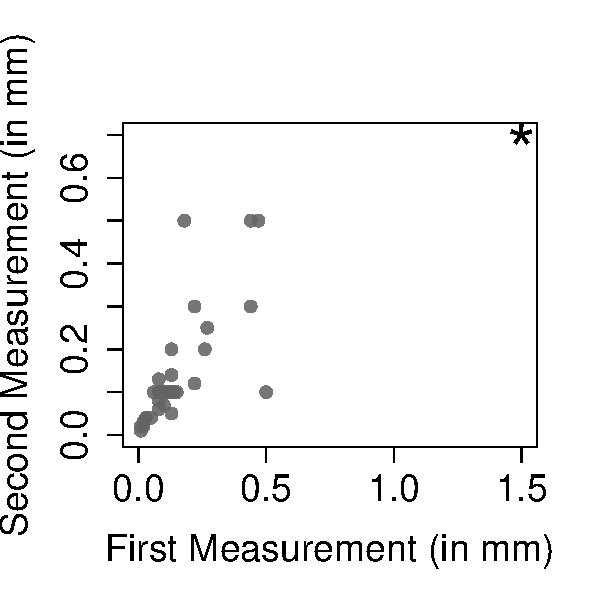
\includegraphics{includes/Item32_R.pdf}
\end{marginfigure}
 
\begin{enumerate}[leftmargin=1cm, itemsep=.2em]
\item Describe the distribution.
\item \replaced{What effect does the starred point have on the correlation?  That is, if the starred point were removed, how would be correlation change, if at all?}{Estimate the correlation with and without the starred point.}
\end{enumerate}

\subsection{\textbf{\textit{Item 33}}}
A study in the \textit{Journal of Leisure Research} investigated the relationship between academic performance and leisure activities.  Each in a sample of 159 high-school students was asked to state how many leisure activities they participated in weekly.  From the list, activities that involved reading, writing, or arithmetic were labeled ``academic leisure activities.'' Some of the results are in the table below:

\begin{table}[!ht]
\begin{center}
\begin{tabular}{lrr}
\hline
& Mean & Standard Deviation\\
\hline
GPA & 2.96 & 0.71\\
Number of leisure activities & 12.38 & 5.07\\
Number of academic leisure activities & 2.77 & 1.97\\
\hline
\end{tabular}
\end{center}
\end{table}

Based on these numbers (and knowing that the GPA is a value between 0 and 4 and the number of activities cannot be negative), discuss the potential skewness of each of the above variables.

\subsection{\textbf{\textit{Item 34}}}
Events A and B are disjoint.  Discuss whether or not A and B can be independent. 

\subsection{\textbf{\textit{Item 35}}}
A sample of 200 mothers and a sample of 200 fathers were taken.  The age of the mother when she had her first child and the age of the father when he had his first child were recorded.

\begin{enumerate}[leftmargin=1cm, itemsep=.2em]
\item Describe the data for the mothers' age.
\item Describe the data for the fathers' age.
\begin{marginfigure}
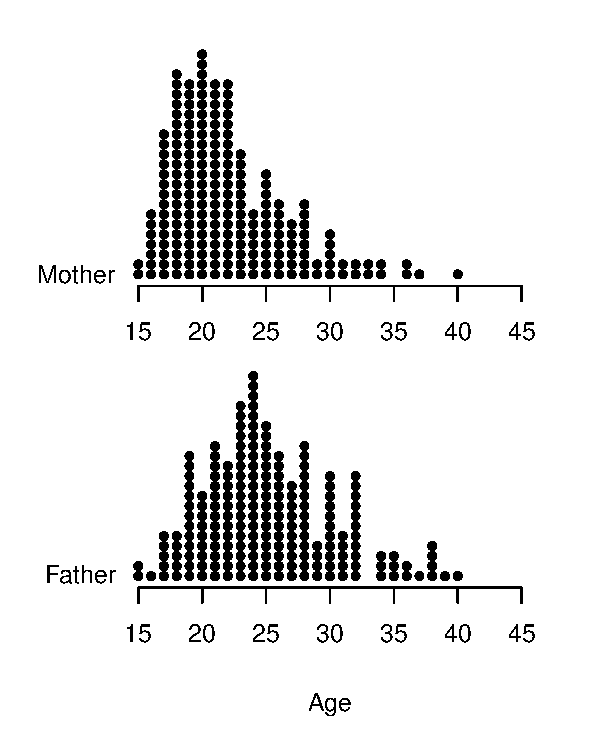
\includegraphics[width=2.75in]{includes/Item35.pdf}
\end{marginfigure}
\item Compare the distributions.
\item A suggestion is made to check the correlation between the ages if we wish to compare the two populations.  Is this a good suggestion?  Why or why not?
\end{enumerate}

\added{\subsection{\textbf{\textit{Item 36}}}
When doing a randomized experiment, the original randomization of units to
treatment groups breaks the association between
\begin{enumerate} [leftmargin=2cm, itemsep=.2em]
\item The explanatory variable and the response variable
\item The explanatory variable and confounding variables
\item The response variable and confounding variables
\end{enumerate}
}

\added{\subsection{\textbf{\textit{Item 37}}}
When doing a randomization test, the simulated re-randomization of units to
treatment groups breaks the association between
\begin{enumerate} [leftmargin=2cm, itemsep=.2em]
\item The explanatory variable and the response variable
\item The explanatory variable and confounding variables
\item The response variable and confounding variables
\end{enumerate}
}

\added{\subsection{\textbf{\textit{New Item 38}}}}
\added{For each of the following, circle your answer to indicate whether the quantity can NEVER be negative or can SOMETIMES be negative:
\begin{enumerate} [leftmargin=1cm, itemsep=.2em]
\item z-score			SOMETIMES		NEVER
\item Probability			SOMETIMES		NEVER
\item Test statistic		SOMETIMES		NEVER
\item Sample proportion		SOMETIMES		NEVER
\item Standard deviation		SOMETIMES		NEVER
\item Inter-quartile range	SOMETIMES		NEVER
\item Standard error		SOMETIMES		NEVER
\item p-value			SOMETIMES		NEVER
\item Slope coefficient		SOMETIMES		NEVER
\item Correlation coefficient	SOMETIMES		NEVER
\end{enumerate}
}

\added{\subsection{\textbf{\textit{New Item 39}}}}
\added{A high school statistics class wants to estimate the average number of chocolate chips in a generic brand of chocolate chip cookies. They collect a random sample of cookies, count the chips in each cookie, and calculate a 95\% confidence interval for the average number of chips per cookie (18.6 to 21.3). Indicate if each is VALID or INVALID.}
\marginnote{\added{Multiple True/False items of this sort that can provide very useful information. If there is a single correct understanding for a statistical concept, but several known misunderstandings for the same concept, a multiple T/F item can provide information on whether or not a student correctly recognizes each of the misunderstandings as false or invalid.}}
\begin{enumerate} [leftmargin=1cm, itemsep=.2em]
\item We are 95\% certain that the confidence interval of 18.6 to 21.3 includes the true average number of chocolate chips per cookie.     VALID   INVALID
\item We are 95\% certain that each cookie for this brand has approximately 18.6 to 21.3 chocolate chips.     VALID   INVALID
\item We expect 95\% of the cookies to have between 18.6 and 21.3 chocolate chips.     VALID   INVALID
\end{enumerate}

\added{\subsection{\textbf{\textit{New Item 40}}}}
\added{Suppose that you have a very big container with 1000 candies in it; 600 are red and 400 are yellow. The candies are all mixed up in the container. With eyes closed, students draw 10 candies, one at a time. They record whether each candy was red or yellow, and then replace and remix the candies. The teacher asked each student to do this six times. Kate, Dana, and Minh decided to play a trick on their teacher. Only one of them actually did the experiment, while the other two just made up their data. Below are their reports, where R = red candy and Y = yellow candy.}
\marginnote{\added{XX Should be featuring distributions of candies as motivation?  Is this consistent with Gould's \emph{Statistics and the Modern Student}?  Should we note that we students are now seeing statistical activities starting in middle school, many of which utilize traditional activities such as M\&M's?}}
\begin{verbatim}
Kate:                Dana:                Minh:
RRYRYRRYYR (6 red)   RYYRRRYRRY (6 red)   RRYRYRRRRY (7 red)
YRRYRRRYRY (6 red)   YRYRRYYRRY (3 red)   RYYYRRRRRR (7 red)
RRYRYRRRYY (6 red)   RRYRRRYRRR (8 red)   YRRRYYRRYY (5 red)
RYRRRYRYRY (6 red)   YRYYYYYYYY (1 red)   RRRRRYRRYR (8 red)
YRRYRRYYRR (6 red)   RRRRRRRRYR (9 red)   RYRRYYYRRR (6 red)
RRRYRYYRYR (6 red)   RYYRYYRRYY (4 red)   YRYRYRRRRR (7 red)
\end{verbatim}
\added{Which student do you think is most likely to have done the experiment?}

\added{\subsection{\textbf{\textit{New Item 41}}}}

\added{Consider an observational study of the effects of second-hand smoke on
health in which we want to compare non-smokers (i) who live with a smoker
to (ii) those who do not live with a smoker. There are two ways in which
independence is relevant in the sampling and data collection process. (a)
Give an example in which one type of independence is met but the other is
not; (b) give an example in which the other type of independence is met but
the first is not.}

\ 

\added{\subsection{\textbf{\textit{New Item 42}}}}

\added{A terse report of a statistical test is given below:
\begin{quote}
The P-value for a hypothesis test with hypotheses $H_0: \mu = 3$ versus $H_1: \mu \neq 3$ is 0.04.
\end{quote}

Critique the following responses for clarity, completeness  and correctness.}

\begin{enumerate} [leftmargin=1cm, itemsep=.2em]
\item This means that the probability of getting our test statistic is .04.

\item This means that the probability of getting a test statistic at least as extreme as ours is .04.

\item This means that if the null hypothesis is true, the probability of getting a test statistics at least as extreme as ours is .04

\item This means that if the null hypothesis is true, the probability of getting a test statistic less than or equal to the one we got is .04

\item This means that it is very unlikely that the result that was used to compute this P-value would have happened by pure chance alone, assuming that  H0 is true. Therefore we could conclude that the evidence is against the Null Hypothesis , and H0 is probably  not true.

\item The sentence means that assuming the population average is equal to three, the likelihood of getting an average as large or larger than we got for our sample is about 4 percent. 

\item The p-value is the probability that the data will be as extreme or more extreme as the alternate hypothesis suggests.
\end{enumerate}


\added{\subsection{\textbf{\textit{New Item 43}}}}

\added{Another exam question asked for an explanation of what the following sentence means:

The interval (2.25, 2.75) is a 99\% confidence interval for the mean GPA of UT students having between 45 and 60 credit hours.

Critique the following responses for clarity and correctness.}

\begin{enumerate} [leftmargin=1cm, itemsep=.2em]
\item A 99\% confidence interval is used to show that 99\% of the time when you pick a sample from the population  (students having between 45 and 60 credit hours) you will find a mean GPA in the interval (2.25, 2.75).

\item This means that 99\% of the confidence intervals we compute using the same method used here will contain the true population men. Or, there is a 99\% chance that $2.25 \leq \mu \leq  2.75$.

\item This means that if we took many, many simple random samples and constructed a confidence interval based on each sample,  99\% of the resulting confidence intervals would contain the true mean.
\end{enumerate}

\added{\subsection{\textbf{\textit{New Item 44}}}}
\added{
For each part, draw a scatter plot satisfying the conditions given, or else explain why the conditions are impossible:}
\begin{enumerate} [leftmargin=1cm, itemsep=.2em]
\item Regression line has small positive slope and correlation is high and positive.
\item Regression line has large positive slope and correlation is high and positive.
\item Regression line has small positive slope and correlation is low and positive.
\item Regression line has large positive slope and correlation is low and positive.
\item Regression line has positive slope and correlation is negative.
\end{enumerate}



\section{\textbf{\added{Examples of Assessments for Presentations and Projects}}}

\added{Projects and presentations are an increasingly 
\marginnote{Halvorsen (ICOTS, 2010, \url{http://iase-web.org/documents/papers/icots8/ICOTS8_4G3_HALVORSEN.pdf} provides motivation for the use of projects as well as details of specific deliverables.}
common component of introductory statistics courses.  
 Projects provide an opportunity for 
students to learn statistics by doing statistics.  They demonstrate that statistical practice includes
formulating a statistical question, designing a plan for collecting relevant data, using appropriate
statistical methods for analyzing the data, and presenting results in a public setting such as a poster,
oral presentation, or a paper (Halvorsen, ICOTS 2010). 
Students have the opportunity to 
to develop statistical questions that arise from broader research questions, to design data
analysis plans, and to communicate results.
We provide a basic rubric for presentations and projects along with a sample numeric grading scheme.}

\added{\begin{tabular}{| p{4cm} | p{4cm} | p{4cm} | p{4cm} |}
\hline
% X & \multicolumn{3}{|c|}{Achievement Level}\\
 Core Competency &  Needs Improvement & Basic & Surpassed \\
 \hline
 \hline		
\textbf{Computation}
Perform computations &
Computations contain errors and extraneous code &
Computations are correct but contain extraneous/unnecessary computations	&
Computations are correct and properly identified and labeled \\
 \hline
\textbf{Analysis}
Choose and carry out analysis appropriate for data and context	 &
Choice of analysis is overly simplistic, irrelevant, or missing key component &
Analysis appropriate, but incomplete, or not important features and assumptions not made explicit &
 Analysis appropriate, complete, advanced, relevant, and informative \\
  \hline
\textbf{Synthesis}
Identify key features of the analysis, and interpret results (including context) &
 Conclusions are missing, incorrect, or not made based on results of analysis &
 Conclusions reasonable, but is partially correct or partially complete &
 Make relevant conclusions explicitly connected to analysis and to context \\
  \hline
\textbf{Visual presentation}
Communicate findings graphically clearly, precisely, and concisely  & 
 Inappropriate choice of plots; poorly labeled plots; plots missing &
 Plots convey information correctly but lack context for interpretation &
 Plots convey information correctly with adequate/appropriate reference information \\
  \hline
\textbf{Verbal}
Communicate findings in writing clearly, precisely, and concisely &
 Explanation is illogical, incorrect, or incoherent. &
 Explanation is partially correct but incomplete or unconvincing	&
 Explanation is correct, complete, and convincing \\
 \hline
 \end{tabular}}

\added{If needed, the competencies can be converted into a numeric score. 
One might begin by giving a score of 85 for achieving basic competency in all 5 categories.
Then we add to this score for competencies that surpass the basic level and subtract for 
those that need improvement.
Three points might be added (subtracted) for each of the first three competencies that 
have surpassed the basic (need improvement), with
four points added (subtracted) for the fourth competency that is surpassed (needs improvement) 
and five points for the fifth competency. 
In other words, it is increasingly challenging to surpass the basic competency, 
and it is increasingly problematic to not achieve basic competency.
For example, if all five competencies
are rated ``surpassed", the score is $85 + 3*3 +4 + 5 = 100$; 
if 4 competencies are rated ``surpassed" and the fifth is ``basic" then the score is $85 + 3*3 +4 = 95$;  and for 3  ``surpassed", 1 
``needs improvement", and 1 ``basic", the score is $85 + 3*3 - 3 = 91$.
If a competency is missing, then 15 points are subtracted regardless of how many 
competencies are categorized as needing improvement.}
